\subsection{Der Block-Editor}

Es wurde sich für die Entwicklung einer Low-Code-Oberfläche entschieden, in der einzelne Elemente als Blöcke dargestellt werden. Wie diese bei der Bearbeitung von Konvertierungen aussieht, ist in Abbildung \ref{fig:buffet-simple} zu sehen. Der Informationsfluss wurde von links nach rechts konzipiert, sodass links die Ausgangsdaten zu finden sind, die rechts eingetragen werden können.

Im linken Bereich befinden sich sowohl die abfragbaren Tabellenspalten (als "Abfragbare Felder" bezeichnet), als auch Funktionen. Über diesen beiden Abschnitten sind Schaltflächen zum Filtern untergebracht, sodass die abfragbaren Felder oder Funktionen wahlweise ausgeblendet werden können. Die Elemente werden als große Schaltflächen dargestellt und enthalten relevante Informationen: Der Datentyp wird als Text (grau, oben links) und als Symbol (rechts) angezeigt. Bei Funktionen handelt es sich hierbei um den Rückgabetyp. Abfragbare Felder weisen ihre Namen und Schlüssel auf (z.B. "Bevölkerung" und "bevoelkerung"), während Funktionen über einen Namen und eine Beschreibung verfügen (z.B. "=" und "Gleichheitsprüfung"). Durch diese Auflistung soll das Nachschlagen und Eintippen von Elementen durch ein einfaches Auswählen ersetzt werden.

\begin{figure}[ht]
  \centering
  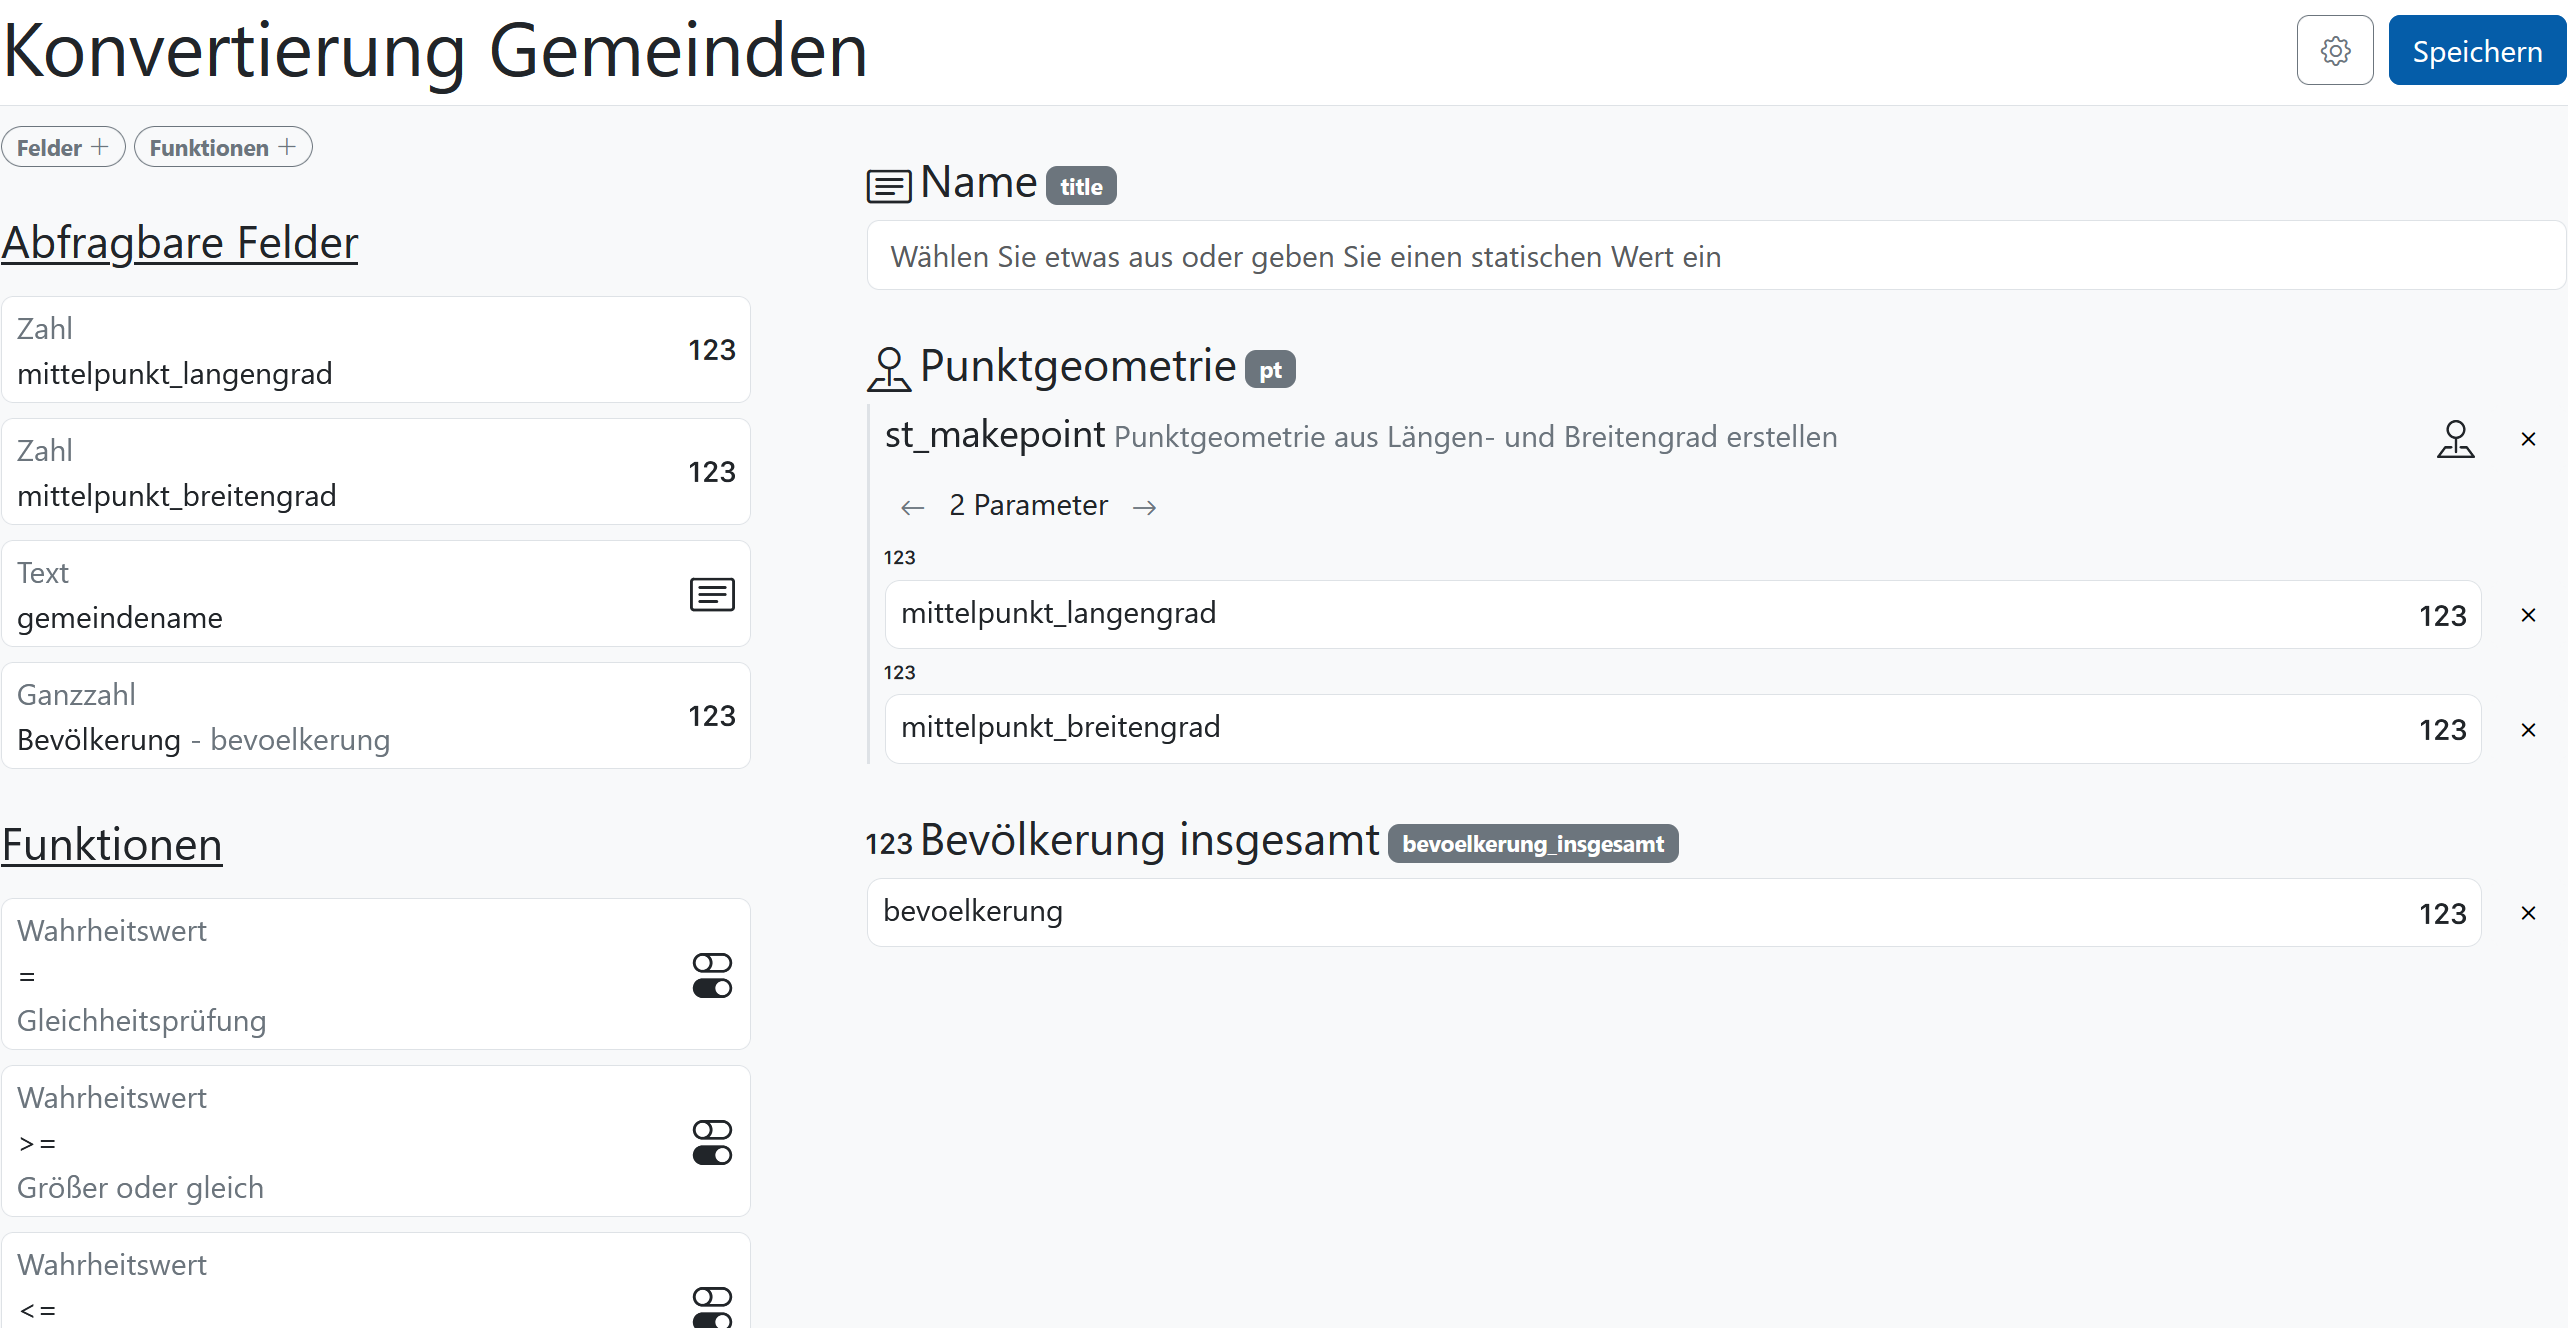
\includegraphics[width=.95\textwidth]{assets/buffet-simple.png}
  \caption{Verwendung des Block-Editors zur Erstellung einer Konvertierung der Klasse "Gemeinde"}
  \label{fig:buffet-simple}
\end{figure}

Im rechten Bereich der Oberfläche wird die Zielstruktur dargestellt. Bei Konvertierungen wird diese durch die Klassendefinition vorgeschrieben. Die Eingabemaske für die einzelnen Attribute besteht aus einem Symbol für den Datentyp, dem Attribut-Name und -Schlüssel, sowie einem dem Datentyp angepassten Eingabefeld. Sobald ein Eingabefeld mit einer Auswahl befüllt wurde, besteht die Möglichkeit, diese wieder durch die Schaltfläche am rechten Rand zu entfernen. Falls das Feld durch eine Funktion gebildet werden soll, muss zuerst die Funktion ausgewählt werden, wodurch wiederum zu Parametern korrespondierende Eingabefelder entstehen. Diese können dann analog mit Attributen oder Funktionen befüllt werden. Somit ist es möglich, beliebig komplexe Schachtelungen zu erstellen\footnote{Eine Obergrenze für den Grad der Schachtelung könnte maximal durch begrenzten Bildschirmplatz erreicht werden. Da pro Schachtelung nur wenig horizontaler Platz verloren geht, wird angenommen, dass diese Grenze höher liegt, als in der Praxis benötigt.}. Die Zusammengehörigkeit von Parametern und Funktionen wird durch einen vertikalen Strich an der linken Seite dargestellt. Abbildung \ref{fig:buffet-scenario} zeigt, wie dies mit einer komplexeren Abfrage aussieht.

\begin{figure}[ht]
  \begin{center}
    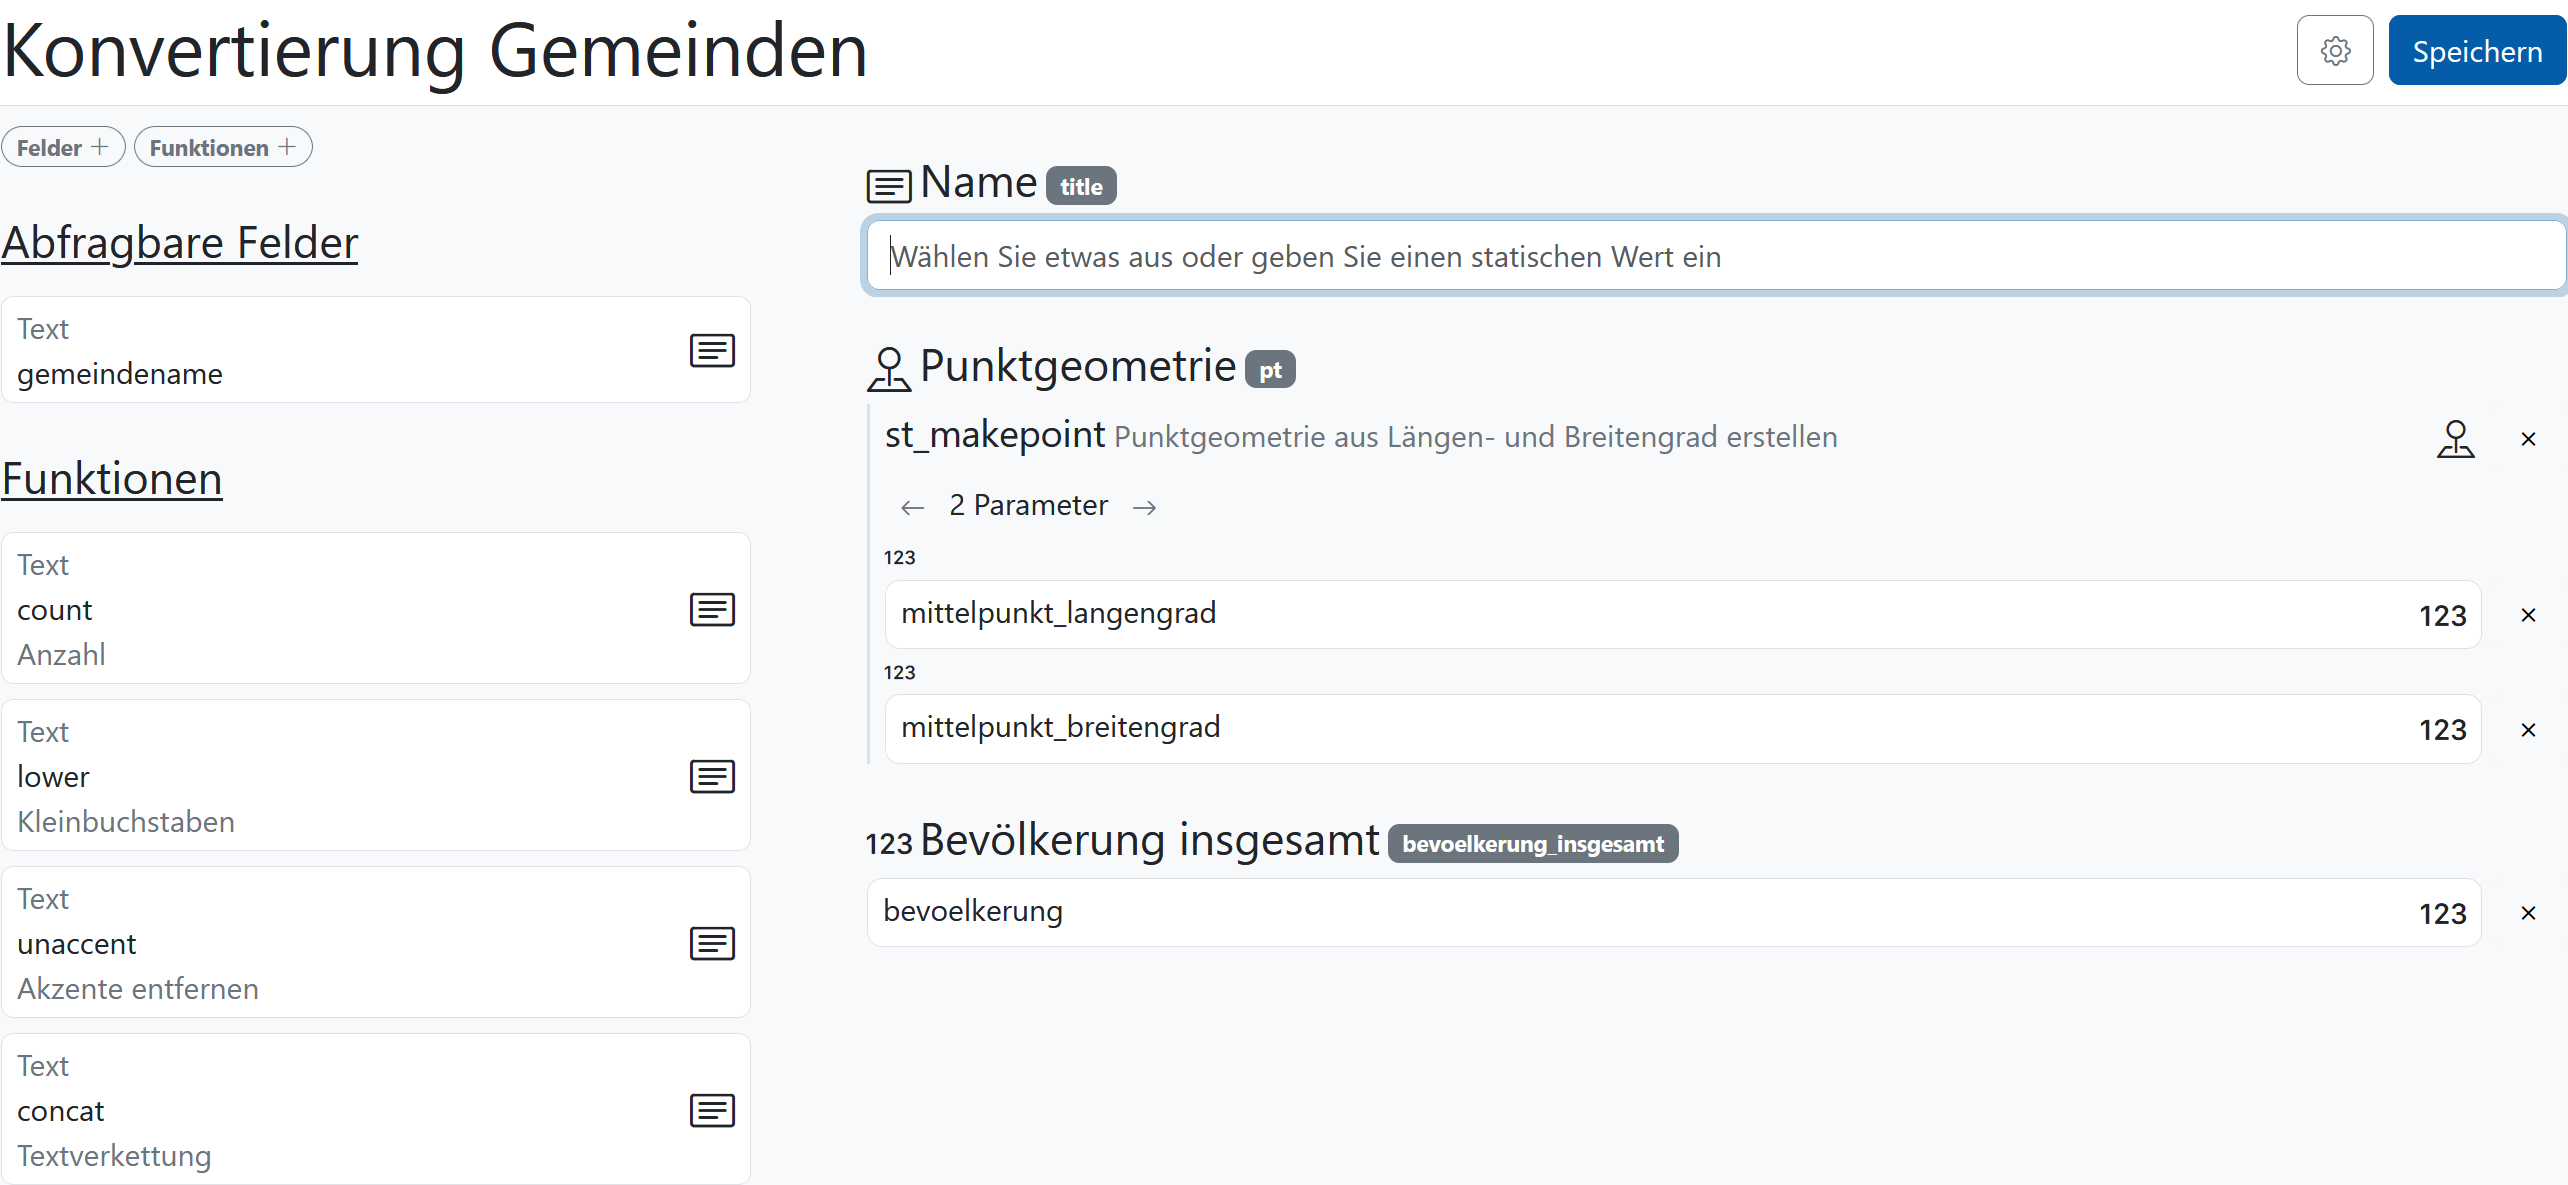
\includegraphics[width=.95\textwidth]{assets/buffet-selected.png}
  \end{center}
  \caption{Erstellung einer Konvertierung der Klasse "Gemeinde", das Feld "Name" ist ausgewählt.}
  \label{fig:buffet-selected}
\end{figure}

Die dargestellten Datentypen erfüllen nicht nur eine informative Funktion, sondern sind auch inhaltlich relevant. Felder können nur mit Elementen befüllt werden deren Datentyp übereinstimmt. Somit soll ein Minimum an Korrektheit der Abfragen sichergestellt werden. Außerdem wird diese Einschränkung dazu genutzt, die Zuordnungsmöglichkeiten zu reduzieren. Wird auf das zu einem Attribut gehörige Eingabefeld geklickt, wird der Auswahlbereich links auf Elemente des Datentyps des Attributs gefiltert. Dies ist anhand des Attributs "Name" in Abbildung \ref{fig:buffet-selected} zu sehen. Umgedreht ist es auch der Fall: Wird links ein Attribut oder eine Funktion angeklickt, werden rechts die Felder ausgegraut, in die die Auswahl nicht eingefügt werden kann. Somit ist es im entwickelten Editor sowohl möglich, zuerst die Ausgangsdaten auszuwählen oder zuerst das Zielfeld.

\begin{figure}[ht]
  \begin{center}
    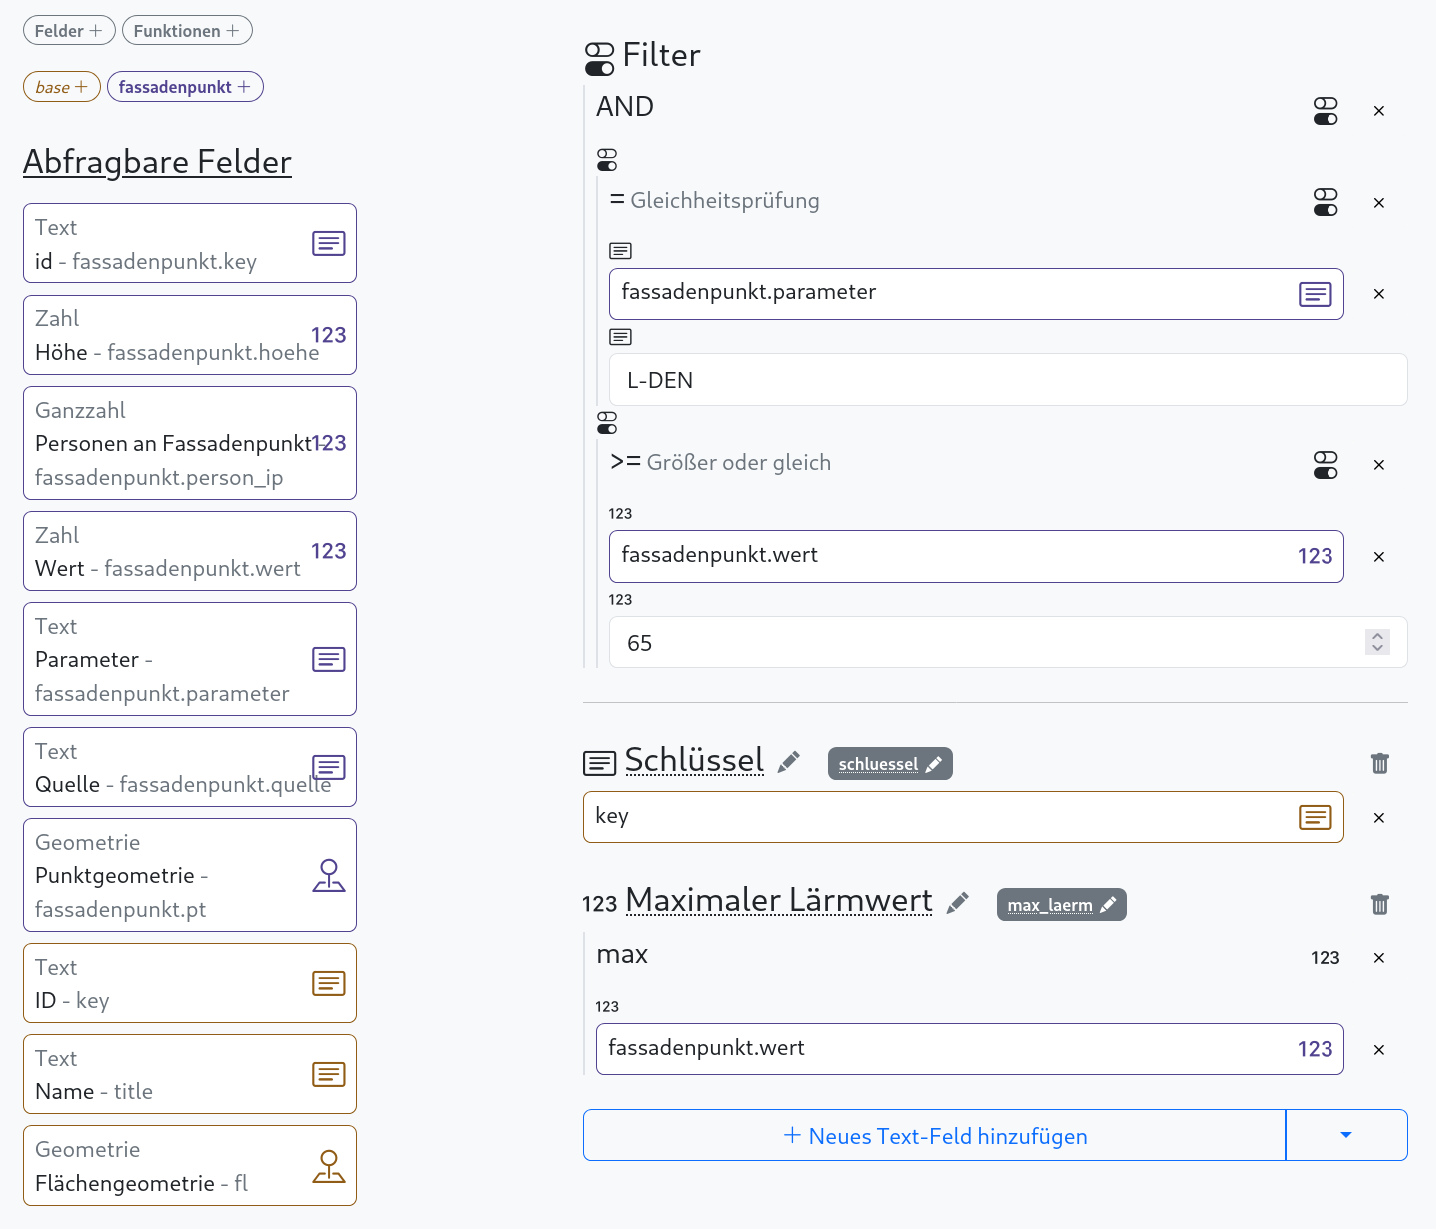
\includegraphics[width=.95\textwidth]{assets/lpz-scenario.png}
  \end{center}
  \caption{Verwendung des Block-Editors zur Erstellung eines SimplexSzenarios.}
  \label{fig:buffet-scenario}
\end{figure}

Der Block-Editor kann auch verwendet werden, um SimplexSzenarios zu erstellen. Dabei werden mehrere Bedienelemente hinzugefügt. In Abbildung \ref{fig:buffet-scenario} wird die Definition eines SimplexSzenarios gezeigt. Dabei wurden zuvor bereits die relevanten Klassen ("Blockseite" und "Fassadenpunkt") ausgewählt. Ein wichtiger Unterschied zu Konvertierungen besteht darin, dass die abfragbaren Felder aus den Attributen mehrerer Klassen bestehen. Diese unterscheiden sich einerseits im Präfix ihrer Schlüssel, andererseits wurde zur schnellen Identifizierung auch eine farbliche Anpassung vorgenommen. Sowohl das Symbol für den Datentyp, als auch die Umrandung sorgen für eine farbliche Sortierung der Objektklassen. Diese Farben werden auch im Kopf des linken Bereichs widergespiegelt, dort kann nun analog zum Elementtyp (Felder oder Funktionen) auch nach Klassen gefiltert werden. Im Beispiel (Abbildung \ref{fig:buffet-scenario}) wird eine fachspezifische Abfrage generiert, die die maximalen Lärmwerte entlang von Blockseiten aggregiert.

Des Weiteren verfügt der Block-Editor im Szenario-Modus über einen Button, um neue Felder hinzuzufügen. Dabei muss bereits der gewünschte Datentyp gewählt werden. Während standardmäßig Felder vom Typ Text hinzugefügt werden, können die anderen Datentypen über ein Dropdown-Menü ausgewählt werden.

Sowohl der Titel als auch der Schlüssel von kreierten Feldern kann bearbeitet werden. Die Darstellung ist die gleiche wie bei Konvertierungen, mit dem Unterschied, dass die editierbaren Informationen gepunktet unterstrichen sind und ein Stift-Symbol daneben angezeigt wird.
